\documentclass[12pt,letterpaper]{article}
\usepackage{fullpage}
\usepackage[top=2cm, bottom=4.5cm, left=2.5cm, right=2.5cm]{geometry}
\usepackage{amsmath,amsthm,amsfonts,amssymb,amscd}
\usepackage{lastpage}
\usepackage{enumerate}
\usepackage{fancyhdr}
\usepackage{mathrsfs}
\usepackage{xcolor}
\usepackage{graphicx}
\usepackage{listings}
\usepackage{hyperref}
\usepackage{subfigure} 

\hypersetup{%
	colorlinks=true,
	linkcolor=blue,
	linkbordercolor={0 0 1}
}

\renewcommand\lstlistingname{Algorithm}
\renewcommand\lstlistlistingname{Algorithms}
\def\lstlistingautorefname{Alg.}

\lstdefinestyle{Python}{
	language        = Python,
	frame           = lines, 
	basicstyle      = \footnotesize,
	keywordstyle    = \color{blue},
	stringstyle     = \color{green},
	commentstyle    = \color{red}\ttfamily
}

\setlength{\parindent}{0.0in}
\setlength{\parskip}{0.05in}

\newcommand{\argmin}{\mathop{\mathrm{argmin}}}
\newcommand{\argmax}{\mathop{\mathrm{argmax}}}
\newcommand{\minimize}{\mathop{\mathrm{minimize}}}
\newcommand{\maximize}{\mathop{\mathrm{maximize}}}
\newcommand{\st}{\mathop{\mathrm{subject\,\,to}}}
\newcommand{\dist}{\mathop{\mathrm{dist}}}

\def\R{\mathbb{R}}
\def\E{\mathbb{E}}
\def\P{\mathbb{P}}
\def\S{\mathbb{S}}
\def\Cov{\mathrm{Cov}}
\def\Var{\mathrm{Var}}
\def\half{\frac{1}{2}}
\def\sign{\mathrm{sign}}
\def\supp{\mathrm{supp}}
\def\th{\mathrm{th}}
\def\tr{\mathrm{tr}}
\def\dim{\mathrm{dim}}
\def\dom{\mathrm{dom}}

% Edit these as appropriate
\newcommand\course{10-725 Convex Optimization}
\newcommand\hwnumber{1}                  % <-- homework number
\newcommand\NetIDa{Zuobai Zhang}           % <-- NetID of person #1
%\newcommand\NetIDb{netid12038}           % <-- NetID of person #2 (Comment this line out for problem sets)

\pagestyle{fancyplain}
\headheight 35pt
\lhead{\footnotesize \course}
%\lhead{\NetIDa\\\NetIDb}                 % <-- Comment this line out for problem sets (make sure you are person #1)
\chead{\textbf{\Large Homework \hwnumber}}
\rhead{\NetIDa \\ \today}
\lfoot{}
\cfoot{}
\rfoot{\small\thepage}
\headsep 1.5em

\begin{document}
	
	\section{Convex Sets}
	\begin{enumerate}[(a)]
	\item {\bf Closed and convex sets.}
	\begin{enumerate}[i.]
		\item For any $y_1, y_2 \in A(S)$, according to the definition of $A(S)$, there exist $x_1, x_2 \in S$ satisfying $A(x_1)=y_1$ and $A(x_2)=y_2$. Since $S$ is a convex set, then for any $t\in(0,1)$ we have $tx_1+(1-t)x_2\in S$. Hence, we have
		\begin{equation}
		ty_1 + (1-t)y_2 
		= tA(x_1) + (1-t)A(x_2)
		= tAx_1 + (1-t)Ax_2 
		= A(tx_1+(1-t)x_2) 
		\in A(S),
		\end{equation} 
		which suggests that $A(S)$ is convex.
		\item For any $y_1, y_2 \in A^{-1}(S)$, according to the definition of $A^{-1}(S)$, there exist $x_1, x_2 \in S$ satisfying $A(y_1)=x_1$ and $A(y_2)=x_2$. Since $S$ is a convex set, then for any $t\in(0,1)$ we have $tx_1+(1-t)x_2\in S$. Hence, we have
		\begin{equation}
		A(ty_1 + (1-t)y_2)
		= tAy_1 + (1-t)Ay_2
		= tA(y_1) + (1-t)A(y_2) 
		= tx_1+(1-t)x_2 
		\in S,
		\end{equation} 
		which implies $ty_1+(1-t)y_2\in A^{-1}(S)$. This follows the definition of convex set.
		
		\item The statement holds true given the fact: If $f$ is a continuous function, then the preimage of a closed set is closed. This can be understood since the linear transformation $A(S)$ is always continuous.
		
		\item Consider the following case. Let
		\begin{equation}
		A = \left[\begin{matrix}
		0 & 0 \cr
		0 & 1
		\end{matrix}\right],\quad
		S = \left\{(x,y) \in \R^2 |y\ge e^x\right\}.
		\end{equation}
		It turns out that $S$ is a closed set, while the image of $S$ under $A$ is $\{0\}\times (0,+\infty)$, which is not closed.
	\end{enumerate}

	\item {\bf Polyhedra.}
	\begin{enumerate}[i.]
		\item Assume that $P=\{x\in \R^n: Ax \preceq b, A\in \R^{m\times n}, b\in\R^m\}$ is a polyhedron. We will prove the closeness and convexity of set $P$.
		
		{\bf Closeness.} Given a point $x \notin P$, then we have $Ax \npreceq b$. There exists an integer $i\in \{1,2,...,m\}$, satisfying $a_i^\top x > b$ where $a_i^\top$ denotes the i-th row of $A$. Let $\epsilon = \frac{1}{2n \max_{j=1,2,...,n} \{|a_{ij}|\}}(a_i^\top x - b)$, then for any point $x' \in O(x,\epsilon)$, we have $a_i^\top x' > b$. Thus, $Ax \npreceq b$, which suggests the complement set of $P$ is open. This reflects the closeness of set $P$.
		
		{\bf Convexity.} For $x_1, x_2 \in P$, we have $Ax_1 \preceq b$ and $Ax_2 \preceq b$. Then, for any $t\in(0, 1)$, we have
		\begin{equation}
		A(t x_1 + (1-t)x_2) 
		= t Ax_1 + (1-t) Ax_2 
		\preceq t b + (1-t) b
		= b.
		\end{equation}
		Hence, $t x_1 + (1-t) x_2 \in P$, which demonstrates the convexity of set $P$.
		
		\item The statement tells us that a projection map takes polyhedra to polyhedra. Obviously, $Q=\{(x,y):x\in P,y=Ax\}$ is a polyhedron. Considering the projection $(x,y)\rightarrow y$ taking $Q$ to $A(P)$, it turns out that $A(P)$ is a polyhedron.
		
	\end{enumerate}
	{\bf Bonus.} Similar to (b, ii.), just consider the set $Q=\{(x,y):x\in P,Ay=x\}$ and take the projection map $(x,y)\rightarrow y$.

	\item Let $S$ denote $\{ Z \in \S^n : 0 \preceq Z \preceq I, \; \tr(Z)=k \}$ and for any $X_1,X_2\in S$ and $t\in(0,1)$, it suffices to prove $0 \preceq tX_1+(1-t)X_2 \preceq I$ and $\tr(tX_1+(1-t)X_2)=k$.
	
	Since $X_1,X_2\in S$, we have $0 \preceq tX_1 \preceq tI$ and $0 \preceq (1-t)X_2 \preceq (1-t)I$. After adding these two inequalities, we will get the first equality. And the second equality can be derived by
	\begin{equation}
	\tr(tX_1+(1-t)X_2)
	= t \; \tr(X_1) + (1-t) \,\tr(X_2)
	= t k + (1-t) k
	=k,
	\end{equation}
	which completes the proof. Also, we can recognize that the {\em Fantope} is the convex hull of $\{ Z \in \S^n :  \lambda_i(Z) \in \{0,1\}, i=1,2,...,n, \; \tr(Z)=k \}$ where $\lambda_i(Z)$ denotes the eigenvalues of $Z$. 
	
	\item Consider the polyhedron $S=\{Ax:x\ge 0\}$. If $b \in S$, then the first statement holds true. And for any $y\in\R^m$, we have $b^\top y = x^\top A^\top y$. If $A^\top y \ge 0$, then $b^\top y \ge 0$ since $x\ge 0$. This conflicts with the second statement. 
	
	On the other hand, if $b \notin S$, then the first statement is false.	
	\end{enumerate}
	
	\newpage
	\section{Convex functions}
	\begin{enumerate}[(a)]
	\item Notice that $f(x)=\min_\sigma \; \sum_{i=1}^{n-1} |x_{\sigma(i)} - x_{\sigma(i+1)}| = x_{\max} - x_{\min}$. Here $\sigma$ is the permutation that permute $x$ in non-decreasing or non-increasing order. Thus, for any $x_1,x_2 \in\R^n$ and $t\in(0,1)$, we have
	\begin{equation}
	f(tx_1+(1-t)x_2) = tx_{1\max} - tx_{1\min} + (1-t)x_{2\max} - (1-t)x_{2\min} = tf(x_1) + (1-t)f(x_2).
	\end{equation}
	
	\item Taking the second derivative of $f$ gives us
	\begin{equation}
	\nabla^2 f(x) = \text{diag}([\frac{1}{x_1^2}, \frac{1}{x_2^2}, ..., \frac{1}{x_n^2}]) \succ 0.
	\end{equation}
	The Hessian matrix of $f$ is positive definite, which suggests $f$ is strictly convex.
	
	\item If the $(\nabla f(x) - \nabla f(y))^\top (x-y) \geq 0$ holds true, then $\nabla f(x)$ is monotonically increasing. Combining with the condition that $f$ is twice differentiable, we conclude that $\nabla^2 f(x) \geq 0$ for any $x \in \dom(f)$. This satisfies the second-order characterization of convex function and indicates $f$ is convex.
	
	Similarly, if $f$ is convex, then $\nabla^2 f \geq 0$, which implies that $\nabla f(x)$ is monotonically increasing. This is equivalent to say $(\nabla f(x) - \nabla f(y))^\top (x-y) \geq 0$.
	 
	\item $f(x) = \frac{1}{x},\quad x>0$
	
	\item 
	
	\item For any $(x_1,t_1),(x_2,t_2)\in\dom(g)$ and any $\alpha \in (0,1)$, we have
	\begin{align*}
	&g(\alpha x_1 +(1-\alpha) x_2, \alpha t_1 + (1-\alpha) t_2)\\ 
	=&\; (\alpha t_1 + (1-\alpha) t_2)\cdot f\left(\frac{\alpha x_1 + (1-\alpha) x_2}{\alpha t_1 + (1-\alpha) t_2}\right) \\
	=&\; (\alpha t_1 + (1-\alpha) t_2)\cdot f\left(\frac{\alpha t_1}{\alpha t_1 + (1-\alpha) t_2} \frac{x_1}{t_1} + \frac{1-\alpha}{\alpha t_1 + (1-\alpha) t_2} \frac{x_2}{t_2}\right)\\
	\le&\; (\alpha t_1 + (1-\alpha) t_2) \cdot \left(\frac{\alpha}{\alpha t_1 + (1-\alpha) t_2} f(x_1) + \frac{1-\alpha}{\alpha t_1 + (1-\alpha) t_2}f(x_2)\right)\\
	=&\; \alpha t_1\cdot f\left(\frac{x_1}{t_1}\right) + (1-\alpha) t_2\cdot f\left(\frac{x_2}{t_2}\right)\\
	=&\; \alpha\cdot g(x_1,t_1) + (1-\alpha)\cdot g(x_2,t_2),
	\end{align*}
	where the inequality is due to the convexity of $f$.
	\end{enumerate}
	\newpage
	\section{Lipschitz gradients and strong convexity}
	\begin{enumerate}[(a)]
		\item 
		{\bf ii. $\Rightarrow$ i.}
		$\nabla f$ is Lipschitz with constant $L$ \\
		$\Rightarrow$ $\|\nabla f(x) - \nabla f(y)\|_2\le L\|x-y\|_2\quad\forall x, y$\\
		$\Rightarrow$ $(\nabla f(x) - \nabla f(y))^\top (x -y)\le \|\nabla f(x) - \nabla f(y)\|_2 \|x-y\|_2\le L\|x-y\|^2_2 \quad \forall x, y$
		
		{\bf i. $\Rightarrow$ iii.}
		
		{\bf iii. $\Rightarrow$ iv.} According to the Lagrange Expansion, for any $x,y$, there exists a $t\in[0, 1]$ such that \begin{equation}
		f(y)=f(x)+\nabla f(x)^\top(y-x) + \frac{1}{2}(y-x)^\top \nabla^2 f\left((1-t)x+ty\right) (y-x)
		\end{equation}
		Since $\nabla^2 f(x) \preceq LI$ for all $x$, we have
		\begin{align}
		f(y)&\le f(x)+\nabla f(x)^\top(y-x) + \frac{L}{2}(y-x)^\top (y-x) \nonumber\\
		&= f(x) + \nabla f(x)^\top (y-x) + \frac{L}{2} \|y-x\|_2^2
		\end{align}
		
		{\bf iv. $\Rightarrow$ ii.} For any $x, y \in \dom(f)$, we have
		\begin{equation}
		f(y)\le f(x) + \nabla f(x)^\top (y-x) + \frac{L}{2} \|y-x\|_2^2
		\end{equation}
		and
		\begin{equation}
		f(x)\le f(y) + \nabla f(y)^\top (x-y) + \frac{L}{2} \|x-y\|_2^2.
		\end{equation}
		Adding the two inequalities, we will obtain
		\begin{equation}
		(\nabla f(x) - \nabla f(y))^\top(x-y) \le L \|x-y\|_2^2
		\end{equation}
		
		\item
		{\bf i. $\Rightarrow$ ii.}
		
		{\bf ii. $\Rightarrow$ iii.}
		
		{\bf iii. $\Rightarrow$ iv.}
		
		{\bf iv. $\Rightarrow$ i.}
		 
	\end{enumerate}
	\newpage
	\section{Solving optimization problems with CVX}
	\begin{enumerate}[(a)]
		\item We have implemented the convex optimization algorithms in Julia with the package Convex.jl\footnote{https://github.com/JuliaOpt/Convex.jl}. 
		\begin{enumerate}[1.]
			\item We first employ the CSV package to load the data provided in toy.csv and then use CVX to solve the problem given in the statement. The objective value obtained at the solution is $199.765$. After that, we plot the original and solution data as images in Fig.~\ref{fig:4a1}. Observe that the shape of circle in the original image has been changed into a more angular one. This may be attributed to the penalty term in the lasso criterion function.
			\begin{figure}[htbp]
				\centering
				\subfigure[Original Image]{
					\begin{minipage}[t]{0.5\linewidth}
						\centering
						
\includegraphics{fig/original.png}
					\end{minipage}%
				}%
				\subfigure[Solution Image]{
					\begin{minipage}[t]{0.5\linewidth}
						\centering
						
\includegraphics{fig/fit.png}
					\end{minipage}%
				}
				\centering
				\caption{Images for Problem (a, 1)}
				\label{fig:4a1}
			\end{figure}
		
			\item This time, we adapt the latter term in the criterion function to a 2-norm and obtain an "isotropic" total variation penalty. This gives us the optimal value $182.205$ and the solution image displayed in Fig.~\ref{fig:4a2}.
			\begin{figure}[htbp]
				\centering
				
\includegraphics{fig/fit2.png}
				\caption{Solution Image for "isotropic" 2d lasso problem}
				\label{fig:4a2}
			\end{figure}
		
			It can be recognized that the solution image for 2-norm lasso looks like a circle more. In spite of this, it still has a darker background compared with the original image due to the penalty term.
		
			\item
			\begin{figure}[htbp]
				\centering
				
\includegraphics{fig/baboon.png}
				\label{fig:baboon}
				\caption{Original Images in baboon.csv}
			\end{figure}
			\begin{figure}[htbp]
				\centering
				\subfigure[$\lambda=1,k=0,\text{opt}=36.6$]{
					\begin{minipage}[t]{0.25\linewidth}
						\centering
						
\includegraphics{fig/output70.png}
					\end{minipage}%
				}%
				\subfigure[$\lambda=1,k=1,\text{opt}=34.7$]{
					\begin{minipage}[t]{0.25\linewidth}
						\centering
						
\includegraphics{fig/output72.png}
					\end{minipage}%
				}%
				\subfigure[$\lambda=1,k=2,\text{opt}=29.2$]{
					\begin{minipage}[t]{0.25\linewidth}
						\centering
						
\includegraphics{fig/output74.png}
					\end{minipage}%
				}
				\subfigure[$\lambda=1,k=3,\text{opt}=22.6$]{
					\begin{minipage}[t]{0.25\linewidth}
						\centering
						
\includegraphics{fig/output76.png}
					\end{minipage}%
				}%
				\subfigure[$\lambda=1,k=4,\text{opt}=16.7$]{
					\begin{minipage}[t]{0.25\linewidth}
						\centering
						
\includegraphics{fig/output78.png}
					\end{minipage}%
				}%
				\subfigure[$\lambda=1,k=5,\text{opt}=36.6$]{
					\begin{minipage}[t]{0.25\linewidth}
						\centering
						
\includegraphics{fig/output710.png}
					\end{minipage}%
				}
				\subfigure[$\lambda=1,k=6,\text{opt}=11.9$]{
					\begin{minipage}[t]{0.25\linewidth}
						\centering
						
\includegraphics{fig/output712.png}
					\end{minipage}%
				}%
				\subfigure[$\lambda=1,k=7,\text{opt}=8.20$]{
					\begin{minipage}[t]{0.25\linewidth}
						\centering
						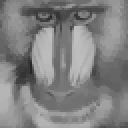
\includegraphics{fig/output714.png}
					\end{minipage}%
				}%
				\subfigure[$\lambda=1,k=8,\text{opt}=3.45$]{
					\begin{minipage}[t]{0.25\linewidth}
						\centering
						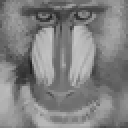
\includegraphics{fig/output716.png}
					\end{minipage}%
				}
			\centering
			\caption{Images for Problem (a, 3)}
			\label{fig:4a31}
		\end{figure}
		\begin{figure}[htbp]
				\centering
				\subfigure[$\lambda=2,k=0,\text{opt}=36.4$]{
					\begin{minipage}[t]{0.25\linewidth}
						\centering
						
\includegraphics{fig/output718.png}
					\end{minipage}%
				}%
				\subfigure[$\lambda=2,k=1,\text{opt}=33.8$]{
					\begin{minipage}[t]{0.25\linewidth}
						\centering
						
\includegraphics{fig/output721.png}
					\end{minipage}%
				}%
				\subfigure[$\lambda=2,k=2,\text{opt}=27.7$]{
					\begin{minipage}[t]{0.25\linewidth}
						\centering
						
\includegraphics{fig/output724.png}
					\end{minipage}%
				}
				\subfigure[$\lambda=2,k=3,\text{opt}=21.1$]{
					\begin{minipage}[t]{0.25\linewidth}
						\centering
						
\includegraphics{fig/output727.png}
					\end{minipage}%
				}%
				\subfigure[$\lambda=2,k=4,\text{opt}=15.3$]{
					\begin{minipage}[t]{0.25\linewidth}
						\centering
						
\includegraphics{fig/output730.png}
					\end{minipage}%
				}%
				\subfigure[$\lambda=2,k=5,\text{opt}=10.8$]{
					\begin{minipage}[t]{0.25\linewidth}
						\centering
						
\includegraphics{fig/output732.png}
					\end{minipage}%
				}
				\subfigure[$\lambda=2,k=6,\text{opt}=7.26$]{
					\begin{minipage}[t]{0.25\linewidth}
						\centering
						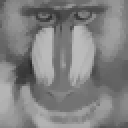
\includegraphics{fig/output734.png}
					\end{minipage}%
				}%
				\subfigure[$\lambda=2,k=7,\text{opt}=4.69$]{
					\begin{minipage}[t]{0.25\linewidth}
						\centering
						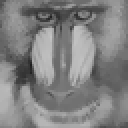
\includegraphics{fig/output736.png}
					\end{minipage}%
				}%
				\subfigure[$\lambda=2,k=8,\text{opt}=2.91$]{
					\begin{minipage}[t]{0.25\linewidth}
						\centering
						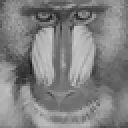
\includegraphics{fig/output738.png}
					\end{minipage}%
				}
				\centering
				\caption{Images for Problem (a, 3)}
				\label{fig:4a32}
			\end{figure}
		\end{enumerate} 
		\item
		\begin{enumerate}[1.]
			\item 
			Since $x>|y|$, we have $\frac{1}{x-y}>0$. So $\frac{1}{x-y}$ and $\frac{1}{(x+y)^2}$ are both convex. Combining with an affine function $z$, these inequalities define a convex set. And this problem is equivalent to the following one:
			\begin{align*}
			\frac{1}{a}+\frac{1}{b^2}-z\le 0,\; a> 0,\;b> 0.
			\end{align*}
			Here, we let $a=x-y$ and $b=x+y$. Since $x>|y|$, we have $a=x-y>0$ and $b=x+y>0$. Thus, the two problems are equivalent.
			\item Here, let $y'=\log y$ and $z'=z^{1/4}$, we will obtain
			\begin{equation*}
			x^2+2e^{-2y'}-5z'\le 0,\; y'>0,\; z'\ge 0.
			\end{equation*}
			Since $x^2$, $e^{-2y'}$ and $-5z'$ are 
		\end{enumerate}
	\end{enumerate}

	{\bf Bonus.}
\end{document}
